\usepackage{booktabs}
\usepackage{caption}
\usepackage{array}

\chapter{Desenvolvimento do Projeto}

Este tópico apresenta informações do produto, desenvolvimento do \textit{software},
tempo para execução, ferramentas utilizadas, viabilidade e riscos.

\section{Métricas}

\begin{table}[!htp]
\centering
\caption{Métricas do projeto}\label{tab: }

\begin{tabular}{l {c} {c} {c} {c} {c} {c} {c} {c}}
\multicolumn{2}{c}{Itens} & \multicolumn{6}{c}{Progresso do Projeto} \\
\cline{2-8}
 & 12/4 & 19/4 & 26/4 & 03/5 & 10/5 & 17/5 & 26/7 \\
\hline
Reuniões & 1 & 2 & 3 & 4 & 5 & 6 & 9 \\
Posts de Blog & 5 & 5 & 6 & 7 & 7 & 7 & 7\\
Vídeos & 1 & 2 & 2 & 2 & 3 & 3 & 3\\
Requisitos & 12 & 12 & 19 & 19 & 19 & 19 & 19\\
Entidades de BD & 0 & 0 & 6 & 6 & 6 & 6 & 6\\
Commits & 3 & 4 & 6 & 9 & 23 & 25 & 30\\
\end{tabular}
\end{table}


\section{Arquitetura da solução}
O projeto web é dividido em duas camadas principais, sendo elas o \textit{front-end}, responsável pela estilização da plataforma e interação com o usuário, e o \textit{back-end}, responsável pela aplicação das regras de negócio, gestão das informações em um banco de dados, e pela lógica de execução em si da plataforma.

 \begin{figure}[!htb]
 	    \centering
 	    \caption{\label{logo}Arquitetura}
 	    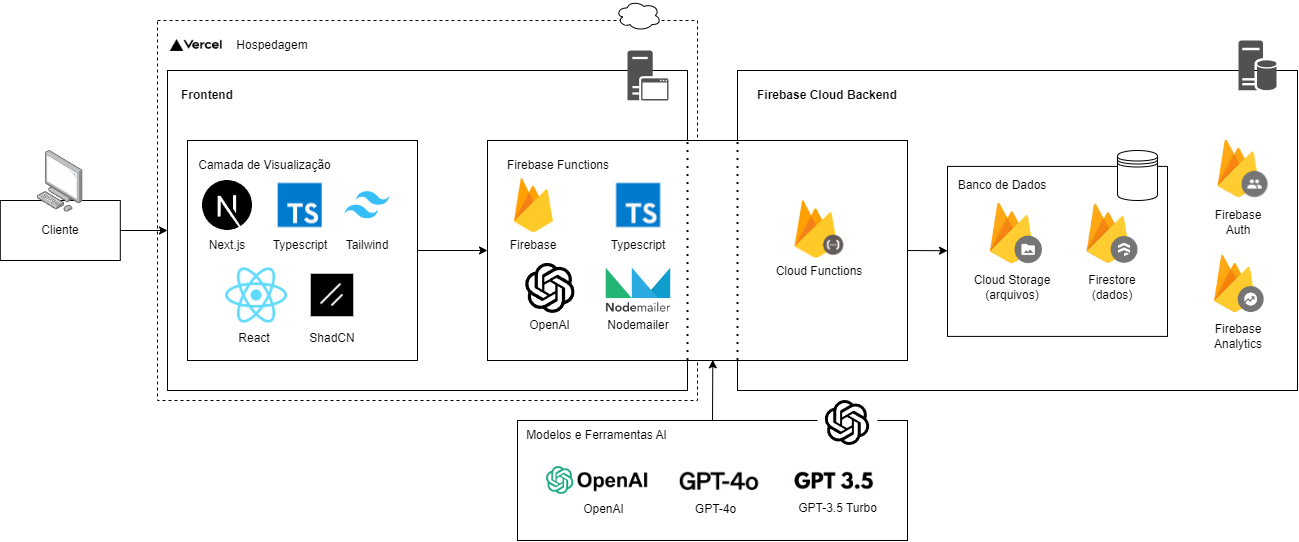
\includegraphics[width=15cm]{img/infra-model.png}
 	    \fonte{Os autores.}
\end{figure}

\subsection{Front-end}
O Front-end é a interface da aplicação, construída com Next.js, um \textit{framework} React que oferece otimizações de desempenho e server-side rendering para uma experiência de usuário mais rápida e fluida. No desenvolvimento da interface, são empregadas as seguintes tecnologias:

\begin{itemize}
    \item \textbf{Tailwind CSS} \newline
Tailwind CSS é uma ferramenta utilizada para a estilização da aplicação. Ele adota uma abordagem de \textit{utility-first}, o que significa que as classes \ac{css} são utilizadas diretamente no \ac{html} para estilizar os elementos. Isso proporciona uma experiência de desenvolvimento mais rápida e consistente, além de facilitar a manutenção do código.

    \item \textbf{ShadCN} \newline
ShadCN é uma coleção de componentes prontos que podem ser importados e customizados dentro do código. Esses componentes são escritos em \textit{Typescript} e Tailwind \acs{css}. Ele não é considerado uma biblioteca, já que é uma extensão do Radix, outra biblioteca de estilização para Javascript.

    \item \textbf{Moment} \newline
Moment.js é uma biblioteca popular para manipulação de datas e horas em JavaScript. Ela oferece uma ampla gama de funcionalidades para formatação, análise e manipulação de datas, tornando mais fácil trabalhar com informações temporais na aplicação.

    \item \textbf{Nodemailer} \newline
Nodemailer é uma biblioteca utilizada para enviar e-mails através de Node.js. Ela oferece uma interface simples e flexível para o envio de \textit{e-mails}, permitindo configurar facilmente o servidor de e-mail, criar templates personalizados e enviar mensagens de forma assíncrona.

    \item \textbf{Framer Motion} \newline
Framer Motion é uma biblioteca de animações para React que facilita a criação de animações fluidas e responsivas em componentes da interface. Ela oferece uma \ac{api} declarativa e intuitiva para definir animações de entrada, saída e transição, além de suportar gestos e interações do usuário.

    \item \textbf{PDF Viewer} \newline
PDF Viewer é uma biblioteca Javascript projetada especificamente para a leitura de arquivos em formato \acs{pdf} enviados pelos usuários, dentro do NodeJS. Com uma série de ferramentas avançadas, oferece uma experiência de visualização personalizada e intuitiva desses documentos.

    \item \textbf{Open AI} \newline
A biblioteca OpenAI permite que os desenvolvedores usem os modelos de \acs{ia} generativos de texto desenvolvidos pela OpenAI, como o GPT 3.5, para criar recursos e aplicativos com tecnologia de \acs{ia}.

    \item \textbf{Bibliotecas do Firebase} \newline
Dentro do \textit{Front-end}, são utilizadas diversas bibliotecas do Firebase para interação com o Back-end e execução de funcionalidades como autenticação, armazenamento de dados e comunicação em tempo real. Algumas das bibliotecas comumente utilizadas incluem:
\begin{itemize}
    \item \textbf{firebase}
    \item \textbf{firebase-admin}
    \item \textbf{firebase-functions}
    \item \textbf{firebase-tools}
\end{itemize}

Essas bibliotecas fornecem uma integração simplificada entre o Front-end e o Back-end, permitindo o desenvolvimento de uma aplicação robusta e interativa.

\end{itemize}

\subsection{Back-end}
Para o Back-end, é utilizado Firebase, que fornece serviços de banco de dados, armazenamento, autenticação e hospedagem, entre outros, de forma simplificada. O Firebase permite uma configuração rápida e fácil, facilitando o desenvolvimento e a viabilização do projeto.
Dentro da plataforma do Firebase, são utilizadas as seguintes funcionalidades:

\begin{itemize}
\item \textbf{Firebase Auth} \newline
Para autenticação de usuários, permitindo login com e-mail, redes sociais, entre outros métodos.
\item \textbf{Firebase Firestore} \newline
Para armazenamento e gerenciamento de dados em tempo real, oferecendo um banco de dados NoSQL escalável e altamente disponível.
\item \textbf{Firebase Storage} \newline
Para armazenamento de arquivos, como imagens e vídeos, diretamente na infraestrutura do Firebase.
\end{itemize}

\subsection{Banco de dados}
O banco de dados da aplicação está contido nos serviços oferecidos pelo Firestore, que é um banco de dados NoSQL escalável e altamente disponível. A comunicação entre as camadas, \acs{api} externas e com o cliente são realizadas através do Protocolo \ac{http} e chamadas \ac{rest}.
O banco de dados é estruturado da seguinte maneira, a fim de suportar a gestão das informações dentro da plataforma:

\begin{itemize}
    \item \textbf{Tabela users}
    
    \begin{itemize}
    \item \textbf{fullname:} Armazena o nome completo do usuário.
    \item \textbf{email:} Guarda o endereço de e-mail do usuário.
    \item \textbf{document:} Pode armazenar o documento de identificação do usuário, como CPF. 
    \item \textbf{noticeid:} Chave estrangeira que faz referência ao edital (notice) associado ao usuário.
    \end{itemize}
    
    \item \textbf{Tabela tasks}
    
    \begin{itemize}
    \item \textbf{title:} Título da tarefa.
    \item \textbf{description:} Descrição detalhada da tarefa.
    \item \textbf{contentid:} Chave estrangeira que referencia o conteúdo (content) associado à tarefa. 
    \item \textbf{difficultyid:} Chave estrangeira que referencia o nível de dificuldade da tarefa. 
    \item \textbf{hasfinished:} Indica se a tarefa foi concluída ou não.
    \item \textbf{userid:} Chave estrangeira que faz referência ao usuário que criou a tarefa. 
    \item \textbf{dayofweek:} Dia da semana em que a tarefa deve ser realizada.
    \item \textbf{startat:} Horário de início da tarefa.
    \item \textbf{finishat:} Horário de término da tarefa.
    \end{itemize}
    
    \item \textbf{Tabela difficulties}
    
    \begin{itemize}
    \item \textbf{name:} Nome do nível de dificuldade.
    \item \textbf{displayname:} Nome de exibição do nível de dificuldade.
    \end{itemize}
    
    \item \textbf{Tabela subjects (matérias)}
    \begin{itemize}
    \item \textbf{name:} Nome da matéria.
    \item \textbf{noticeid:} Chave estrangeira que faz referência ao edital (notice) associado à matéria.
    \end{itemize}
    
    \item \textbf{Tabela contents}
    \begin{itemize}
    \item \textbf{subjectid:} Chave estrangeira que referencia a matéria (subject) associada ao conteúdo. 
    \item \textbf{text:} Texto do conteúdo, que pode conter informações relevantes para estudo.
    \end{itemize}
    
    \item \textbf{Tabela notices (editais)}
    \begin{itemize}
    \item \textbf{name:} Nome do cargo ou edital.
    \item \textbf{filesrc:} Caminho para o arquivo do edital. 
    \item \textbf{userid:} Usuário que fez o upload do edita.
    \end{itemize}
    
\end{itemize}

Este modelo de banco de dados é projetado para permitir a associação de usuários a tarefas específicas, associadas a conteúdos de estudo e matérias específicas relacionadas aos editais. A inclusão de um nível de dificuldade (na tabela difficulties) proporciona uma maneira de classificar a complexidade das tarefas, enquanto a tabela notices permite o armazenamento e acesso aos editais relacionados aos estudos.

 \begin{figure}[!htb]
 	    \centering
 	    \caption{\label{logo}Modelo de classes do banco de dados}
 	    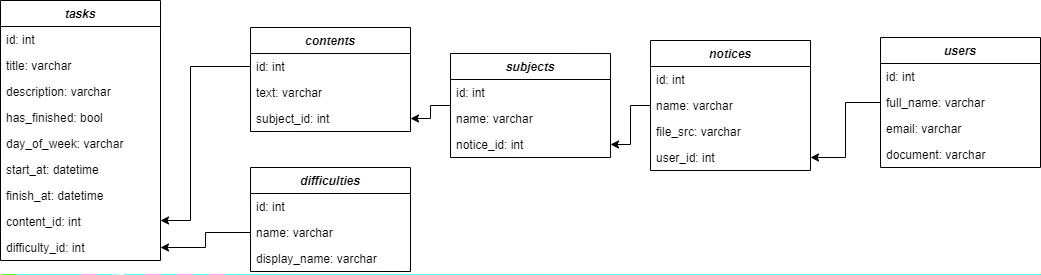
\includegraphics[width=15cm]{img/db-model.png}
 	    \fonte{Os autores.}
\end{figure}
\FloatBarrier

\subsection{Integrações}
Para a interpretação dos conteúdos pragmáticos dentro dos editais, faremos uso dos modelos de inteligência artificial fornecidos pela OpenAI. A OpenAI é uma organização de pesquisa em \acs{ia} conhecida por seus avançados modelos de \acs{ia}, especialmente na área de  \ac{nlp}. Iremos utilizar esses modelos para desenvolver os seguintes motores:

\begin{itemize}
\item \textbf{Interpretação de Conteúdo de Edital e Geração de Matérias} \newline
Este motor é encarregado de interpretar o conteúdo pragmático após a filtragem do edital fornecido pelo usuário. Ele irá identificar e extrair as matérias que serão cobradas no concurso, populando assim o banco de dados.

\item \textbf{Interpretação de Matérias e Geração de Tarefas e Rotinas de Estudo} \newline
 Com o banco de dados já contendo as matérias identificadas, este motor entra em ação para gerar tarefas e rotinas de estudo personalizadas. Recebendo como entrada as matérias e conteúdos que o usuário ainda precisa estudar, ele irá gerar um cronograma de estudo detalhado, distribuindo as tarefas ao longo da semana de acordo com as necessidades e preferências do usuário.
\end{itemize}

Essas integrações permitem uma abordagem mais eficiente e personalizada no processo de estudo para concursos, aproveitando o poder dos modelos de linguagem avançados fornecidos pela OpenAI.

\subsection{Versionamento de Código}
O versionamento de código é uma prática fundamental no desenvolvimento de software, permitindo o controle e gerenciamento das alterações feitas ao longo do tempo em um projeto. Para isso, utilizaremos o \textit{GitHub} como plataforma de versionamento, que oferece uma série de recursos poderosos para colaboração e controle de versões. No nosso ambiente de desenvolvimento, teremos um repositório principal hospedado no \textit{GitHub}:

\textbf{Repositório do \textit{Front-end} e \textit{Functions} do Firebase:} \newline
Este repositório conterá o código-fonte do \textit{Front-end} desenvolvido com \textit{Next.js}, bem como as \textit{Functions} do Firebase utilizadas no Back-end. Será organizado de forma a separar claramente os diretórios relacionados ao Front-end e às functions do Firebase, mantendo uma estrutura de pastas intuitiva e coesa.

\textbf{Estratégia de Versionamento: Gitflow} \newline
Para gerenciar as diferentes etapas de desenvolvimento e garantir uma colaboração eficiente entre os membros da equipe, adotaremos a estratégia de versionamento \textit{Gitflow}. Essa abordagem define um modelo de fluxo de trabalho baseado em branches, que facilita a organização das funcionalidades em desenvolvimento, testes e produção.
Principais \textit{Branches}:

\begin{itemize}
\item \textbf{Main:} Esta \textit{branch} representa a versão estável e de produção do código. Todo o código que está pronto para ser implantado em ambiente de produção é mesclado nesta \textit{branch}.

\item \textbf{Develop:} Esta \textit{branch} é onde o desenvolvimento ativo ocorre. É a \textit{branch} de integração para novas funcionalidades e correções de bugs. Todo o desenvolvimento é feito a partir desta \textit{branch}.

\item \textbf{Feature Branches:} Para cada nova funcionalidade ou tarefa, uma nova \textit{branch} de \textit{feature} é criada a partir da \textit{branch develop}. Esta \textit{branch} é utilizada para implementar a funcionalidade de forma isolada, antes de ser integrada de volta à \textit{branch develop}.
\end{itemize}
 
Adotando essa estratégia de versionamento com o \textit{Gitflow}, garantimos um desenvolvimento organizado, facilitando a colaboração entre os membros da equipe e mantendo um histórico claro e estruturado das alterações feitas no código-fonte ao longo do tempo.

\subsection{Infraestrutura}
Para hospedagem, optaremos por utilizar os serviços especializados de hospedagem da Vercel para o \textit{Front-end} e do Firebase para o \textit{Back-end} customizado.

\textbf{Hospedagem do Front-end} \newline
A Vercel oferece um serviço de hospedagem altamente escalável e otimizado para aplicações \textit{Front-end}, como o nosso desenvolvido com \textit{Next.js}. Utilizando a plataforma da Vercel, podemos implantar e hospedar facilmente nosso Front-end, garantindo uma experiência de usuário rápida e confiável.

\textbf{Hospedagem do \textit{Back-end} no Firebase} \newline
O Firebase oferece por padrão a hospedagem de seus serviços diretamente em sua plataforma, eliminando a necessidade de recorrer a soluções terceirizadas para essa finalidade. Essa integração nativa proporciona uma infraestrutura completa e integrada, capaz de suportar todas as necessidades de nossa aplicação de forma eficiente e escalável.

\subsection{Escalabilidade}
Tanto a Vercel quanto o Firebase oferecem opções de escalabilidade conforme as necessidades do projeto. No caso da Vercel, podemos facilmente escalar nossa aplicação \textit{Front-end} de acordo com o aumento da demanda de tráfego. Já o Firebase, além de oferecer hospedagem escalável, também permite dimensionar automaticamente o banco de dados e outros serviços conforme necessário.

\subsection{Convenções e Padronização de Código}

Convenções são acordos ou regras estabelecidas para padronizar a forma como realizamos determinadas atividades ou interações. No contexto do desenvolvimento de \textit{software}, as convenções de codificação são diretrizes estabelecidas para padronizar a escrita e a organização do código-fonte de uma aplicação. Elas definem como devemos nomear variáveis, formatar o código, documentar funcionalidades e adotar certas práticas de desenvolvimento.

Para esse projeto, iremos seguir com as seguintes convenções e padrões de código:

\begin{itemize}
    \item Nomenclatura de Variáveis e Funções:

Utilize nomes descritivos e significativos para variáveis e funções.
Prefira \textit{camelCase} para nomes de variáveis e funções em \textit{JavaScript/TypeScript}.

    \item Comentários:
Inclua comentários claros e concisos para explicar trechos de código complexos ou de difícil compreensão.
Evite comentários óbvios que apenas repetem o que o código faz.

    \item Indentação e Formatação:

Utilize uma tabulação consistente para indentação, preferencialmente com 2 ou 4 espaços.
Mantenha linhas de código com até 80-100 caracteres para facilitar a leitura em telas menores.
Organize o código de forma clara e coesa, utilizando espaços em branco para separar blocos lógicos.

    \item Tratamento de Erros:

Sempre inclua tratamento de erros adequado em pontos críticos do código.
Utilize \textit{try-catch} para capturar e lidar com exceções de forma apropriada.

    \item Gerenciamento de Dependências:

Mantenha uma lista atualizada de todas as dependências e suas versões no arquivo de manifesto (como \textit{package.json}).
Utilize um gerenciador de dependências confiável, como \acs{npm} ou \acs{yarn}, e evite adicionar dependências desnecessárias.

    \item Revisões de Código:

Realize revisões de código regulares entre os membros da equipe para identificar e corrigir problemas de qualidade, estilo e desempenho.
Mantenha um ambiente colaborativo e aberto para sugestões e melhorias no código.

\end{itemize}

\newpage

